
\documentclass[11pt,a4paper]{article}
    \usepackage[hyperref]{naaclhlt2019}
    \usepackage{times}
    \usepackage{latexsym}
    \usepackage{graphicx} 
     \usepackage{booktabs}
    \usepackage{url}
    
    \aclfinalcopy 
    
    \title{Lyrical Distinction}

    \author{Jesse Bartola \\
      {\tt jbartola@} \\\And
      Phillip Michalowski \\
      {\tt pmichalowski@ } \\\And
      Nischal Tamang \\
      {\tt ntamang@} \\\And
      Max Berezin \\
      {\tt mberezin@} \\}
      
    % \setlength\textwidth{16.0cm}
    \date{}
    
    \begin{document}
    \maketitle
    
    \section{Problem statement}
    Music is an important part of our everyday lives. Technological advances in modern society have made it easier than ever for new artists to distribute their songs over the Internet. Unfortunately, the massive volume of songs that are regularly released into the public can make it difficult to discern which song is made by which artist. Moreover, a more important question arises: Are the most popular artists the ones with the most distinct music?

Aside from sound, the words an artist uses in a song are perhaps the most important determining factor in how it will appeal to the public. Lyrics contain semantic relevance, which allows for the possibility of implicit analysis of a song’s cultural relevance. Some of the greatest artists of all time are renown for their unique use of lyricism. Our project will aim to determine if:
\begin{center}
\small{
(a) Given a set of lyrics, who the artist is with a high-degree of certainty.
\\
(b) Given our trained prediction model, what the lyrical uniqueness rank for various artists is.
}
\end{center}

    
    \section{Our Dataset}
For the implementation of our described methodology, we chose to initially use a Kaggle sourced CSV file for our dataset \newcite{website:Mousehead}. This dataset contains a repository of 57,650 songs of a multitude of artists and genres. The distribution of artists and songs can be seen in Figure \ref{fig:songs_per_artist_I}, which uses a Pareto Distribution to visualize how close to 80\%  of the content within this dataset is described by only around 20\% of the artists. 

\begin{figure}[t]
    \centering
    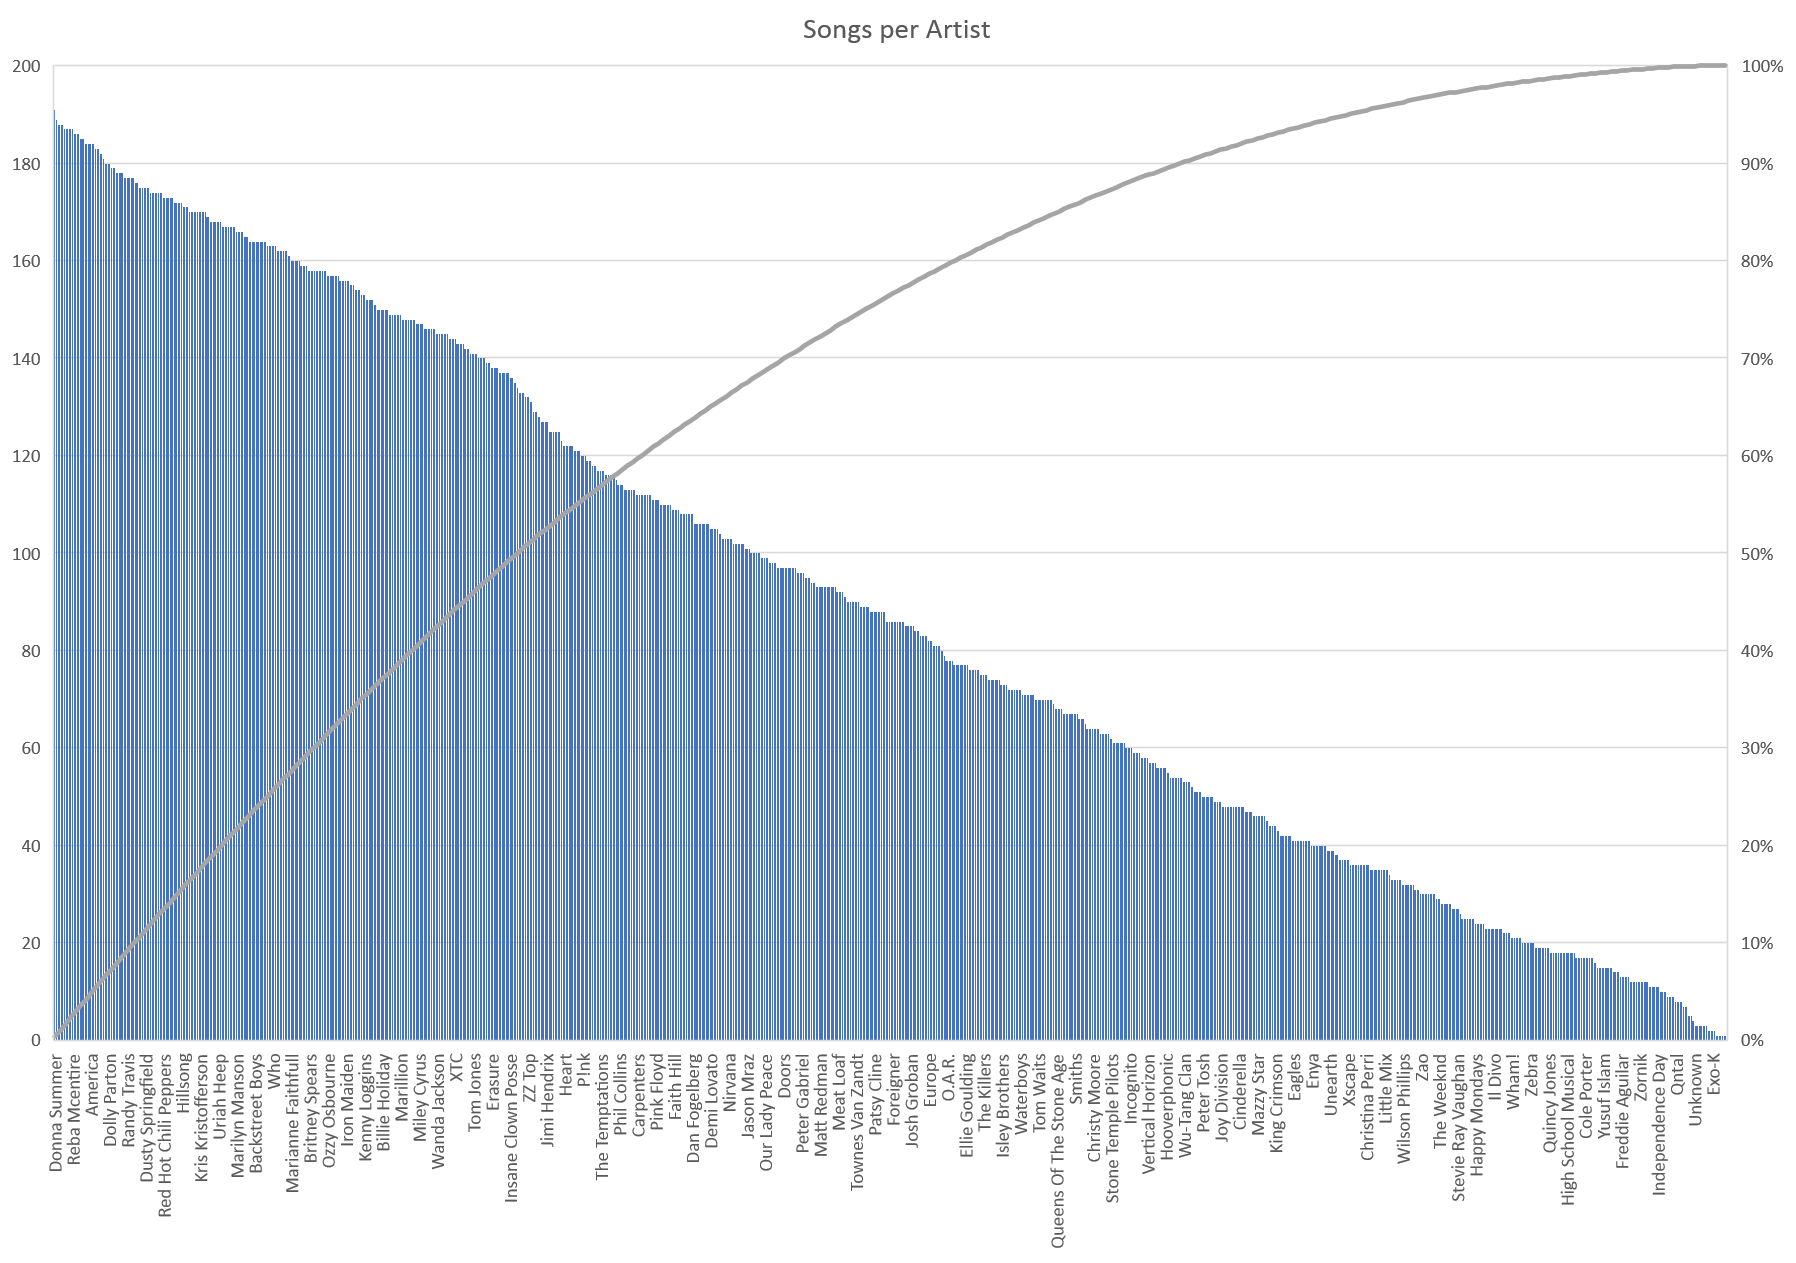
\includegraphics[width=0.5\textwidth]{figs/songs_per_artist_I.png}
    \caption{Songs per Artist: \newcite{website:Mousehead}}
    \label{fig:songs_per_artist_I}
\end{figure}


The column values of the dataset are 
\begin{center}
\textit{artist, song, link, text}
\end{center}
In this schema, the column \textit{text} contains the important lyrical information pertaining to the current song and artist. 

\begin{figure}[t]
    \centering
    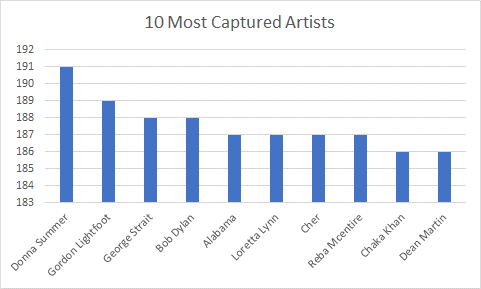
\includegraphics[width=0.5\textwidth]{figs/artists.png}
    \caption{Most Captured Artists: \newcite{website:Mousehead}}
    \label{fig:artists}
\end{figure}

\begin{table}[]
\centering
\begin{tabular}{lllll}
\multicolumn{1}{l|}{} & \multicolumn{1}{l|}{\textit{Average}} & \textit{Std. Dev} &  &  \\ \cline{1-3}
\multicolumn{1}{l|}{Songs Per Artist} & \multicolumn{1}{c|}{94} & \multicolumn{1}{c}{49} &  &  \\ \cline{1-3}
\multicolumn{1}{l|}{Word Count [Fig:\ref{fig:words_per_song}]} & \multicolumn{1}{c|}{219.48} & \multicolumn{1}{c}{108.81} &  &  \\
 &  &  &  & 
\end{tabular}
\caption{Dataset Statistics}

\end{table}

For our future implementations, we plan on using \newcite{website:Kaggle} with 362,237 songs for both its expanded amount of lyrical content.
The column values of this dataset are :
\begin{center}
\textit{index, song, year, artist, genre, lyrics}
\end{center}
This allows us to utilize the additional song information for enahnced modeling (i.e Genre, Year).

\begin{figure}[t]
    \centering
    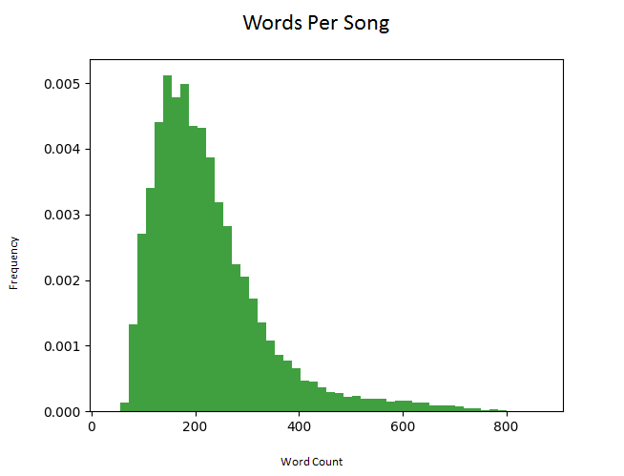
\includegraphics[width=0.5\textwidth]{figs/words_per_song.png}
    \caption{}
    \label{fig:words_per_song}
\end{figure}
    
    \section{Baselines}
For our baseline approach, we used a simple averaging model. We first created a word matrix W. Each row in the matrix W contains the pre-trained GloVe embedding \newcite{pennington2014glove} for a corresponding word in a song. 
A song vector is then computed by calculating the mean of each value in the row of matrix W. 
This vector thus acts as a unique representation for a particular song. 
For a particular artist, a songs matrix S is created. Each row in the matrix S contains all of the different song vectors for that artist. 
We then averaged the values of each row in matrix S to compute the final artist vector. 

\begin{figure}[t]
    \centering
    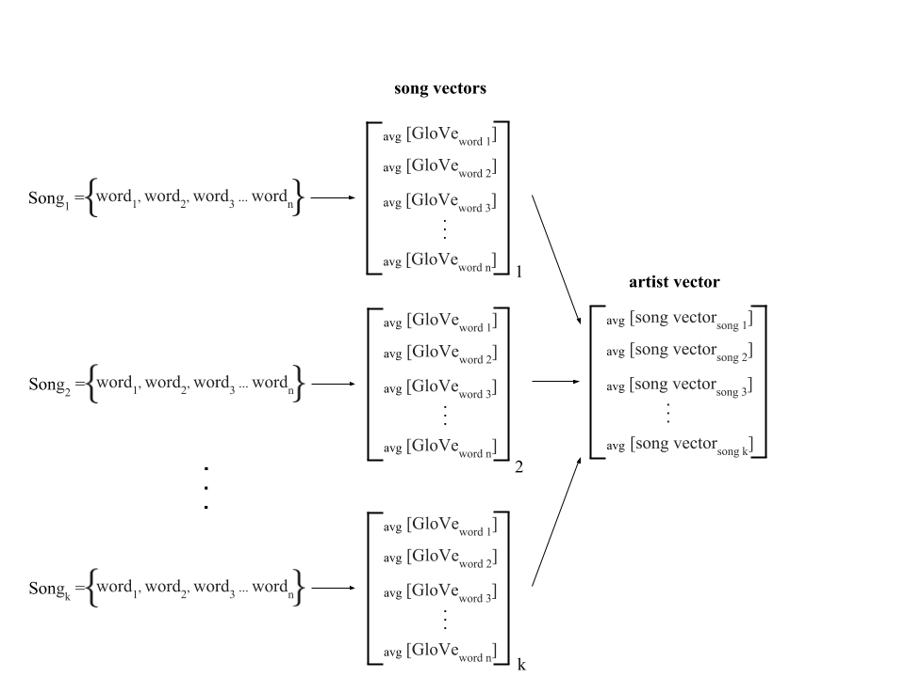
\includegraphics[width=0.5\textwidth]{figs/naive_model.png}
    \caption{Initial Approach}
    \label{fig:naive}
\end{figure}
\begin{figure}[ht]
    \centering
    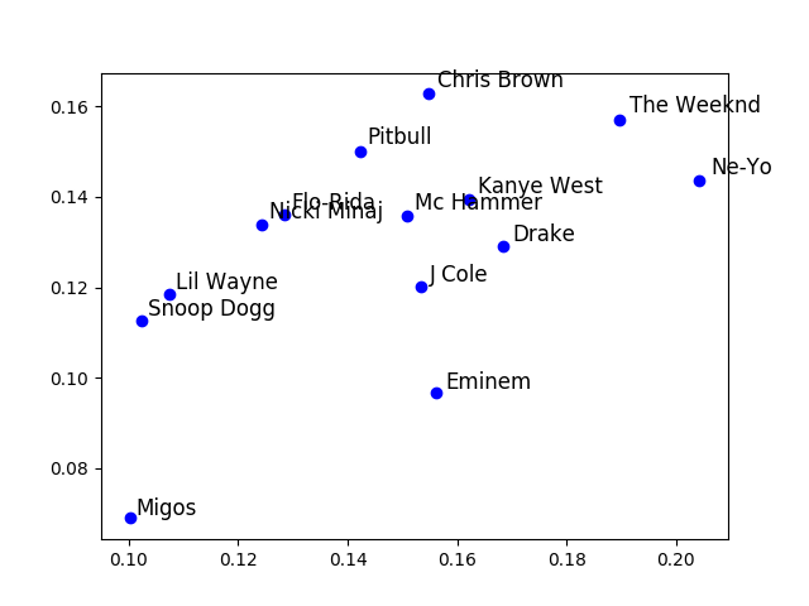
\includegraphics[width=0.5\textwidth]{figs/artist_dist.png}
    \caption{Artist Embeddings Mapped to 2-Dimensions}
    \label{fig:artist}
\end{figure}


After completing these steps for every artist in the dataset, each artist is represented as a single vector embedding [\ref{fig:naive}].

\begin{table}[]
\centering
\begin{tabular}{lllll}
\multicolumn{1}{l|}{} & \multicolumn{1}{l|}{\textit{Cos}} & \textit{Euclidean} &  &  \\ \cline{1-3}
\multicolumn{1}{l|}{k = 1} & \multicolumn{1}{c|}{7.78\%} & \multicolumn{1}{c}{6.69\%} &  &  \\ \cline{1-3}
\multicolumn{1}{l|}{k = 10} & \multicolumn{1}{c|}{21.31\%} & \multicolumn{1}{c}{18.51\%} &  &  \\ \cline{1-3}
\multicolumn{1}{l|}{k = 50} & \multicolumn{1}{c|}{41.99\%} & \multicolumn{1}{c}{40.28\%} &  &  \\

\end{tabular}
\caption{Cos vs. Euclidean Distance Accuracy}
\label{table:similarity_table}


\end{table}

We created a 80/20 train and test split. We tested the model accuracy by taking a lyric from the test set and creating the artist vector embedding with the steps outlined previously. The k closest vectors measured by cosine similarity to the newly generated artist vector is extracted from the learned embeddings. If the correct artist is contained in the top k vectors, we considered it a correct prediction by the model. We chose k to be 10 since it is a fairly low percent of the 643 total artists in the dataset. The model performed at an accuracy of 21.31\%. 

Regarding the vector similarity testing, we experimented both cosine and euclidean distance. Cosine consistently outperformed euclidean on all k values that we tested. The results are shown in table [\ref{table:similarity_table}].

Using the learned artist embeddings, we also plotted a small subset of artists on a 2D graph [\ref{fig:artist}].


    
    \section{Error analysis}


We hypothesize a few reasons to why the baseline model performs so poorly. One is due to there being the same mapping function between the generation of song vectors and the artist vector. Simply averaging rows of matrices loses the meaning between the artists and songs. Our original dataset is also not robust enough. It contains 643 unique artists and around 55,000 songs. The artist with the most songs in the dataset has only about 200 songs. For our final report, we would like to find a bigger dataset with more songs per artist. In addition, we could also find a another dataset and combine it with the dataset we are already using. After annotating failed examples, one thing we noticed was the dataset we used contains song structure labels such as \textit{"chorus"} or \textit{"verse 1"}.

i.e:


\begin{center}
[ repeat chorus ] 
only wait so long before your flower petals are all 
gone baby i was trying to burn bridges of stone 
. [ repeat chorus ]
\end{center}







We also noticed that all songs the model failed on contained common words in the English language as demonstrated by Zipf’s law. In the future, we should remove the song labels and also the most common English words from the dataset as they do not help distinguish between different songs. 

Regarding the issue of the naive mapping function between matrices, we plan to use Neural Networks to obtain a better performing model. The following section outlines our procedure for the Neural Networks implementation.
    
    \section{Our approach}

\begin{center}
 \href{https://github.com/onocy/nlp_f18/tree/rnn_pandas}{Repository}
\end{center}

\subsection{Introduction}
  Our main approach consisted of building a deep learning model to classify which artist created a song given a string of lyrics. We used the Pytorch package  \newcite{paszke2017automatic} and iterated over several implementations of different neural networks. 

\subsection{Vanilla Neural Network}

The first non-trivial implementation we attempted was a simple network with an input layer, three hidden layers of the same dimension and a softmax output layer. To construct the input, we tokenized a string of lyrics into a list of strings, where each string contains exactly one word.


 Each word in the input list was mapping to its respective word embedding in the \textit{glove.6B.50d.txt} file obtained from Homework 2. The output layer produced a probability distribution over all 643 artist in our original dataset. Before we could start training, we needed a reasonable method of standardizing the input to the network.

\subsection{Input}

We decided to create our input to the network by mapping each word in a song to its respective embedding vector and fixing the number of input words from each song to a constant value. If we made this cutoff too short (say, a maximum of 30 words per song input) it could result in the loss of potentially useful information contained in the rest of the song. If the cutoff value was too large, then much of the training data would be padded with zeros, thus taking up unnecessary memory and adding meaningless values to our inputs.

We approached this situation like any good scientist should, and took a closer look at a histogram of words per song in our dataset [\ref{fig:words_per_song}]. The distribution was right-skewed with the mean around 220 words. After training and testing the network using several different cutoff values, a input length of 300 words seemed to produce the highest test accuracy.


\subsection{Training and Testing} 

Similar to our Baseline model, we used a 80/20 train/test split on the vanilla neural network model. Each training example is a 2-tuple containing a unique integer representing an artist and a fixed-length array of word embeddings corresponding to the lyrics in a song. We standardized the training session to run over 20 epochs, as it seemed like our optimization algorithm had diminishing returns when run for any longer. After each training session, we tested the network on our test data by comparing the element in the output vector with the highest probability to the ground truth value of the artist who created the song.

While training, we adjusted the batch sizes to various powers of 2 (16, 32, 64, 128, and 256) and determined that with other hyperparameters fixed, a batch size of 64 yielded best test accuracy. We experimented using the Adam and SGD optimizers, both of which yielded very similar test results, even when used with different learning rates (ranging from 0.001 to 0.5). 

We tested our network numerous times after training it with different combinations of hyperparameters. The accuracy was appalling each and every time. The maximum value we achieved was a test result of 0.38\% accuracy. After some investigation, we discovered a few reasons for this:

1. We had 643 different output classes, but less than 20 training examples for many artists. The asymmetry of songs per artist potentially biased the network into learning stronger weights for some artists than others

2. Our test method was comparing the output class with the highest probability to the true value of the artist. Given the amount of data we had per class, it would have been more reasonable to check if the ground truth artist was contained in the top k output classes (5 or 10) with highest probability
\\ 

Our poor results in this network led us to try other deep learning implementation that better lend themselves to NLP tasks. Needless to say, vanilla neural network are far from ideal when it comes to tasks involving sequential input.

\subsection{LSTM}   

The second implementation we tried was an LSTM (Long-Short Term Memory) recurrent neural network. \newcite{website:LSTM} networks are much better at extracting information from sequential input and time-series data. This time instead of using the pre-trained embeddings from the glove file, we learned all embedding representations from our dataset by creating an embedding layer and learning them through the training process.

Utilizing the same strategies as we did for the vanilla neural network, we tried different values of each hyperparameter (batch size, optimizer, input size, learning rate, hidden state dimensions, etc.) and found that with a batch size of 64, Adam optimizer, input size of 300, learning rate of 0.05, and 2 hidden states of dimension 10 we achieved an average accuracy of ~60\% over 10 test runs, using k = 30 as a the correctness distance (i.e., the ground truth artist appeared in the 30 highest probabilities in the output distribution, which is 30/643 = ~5\% of out dataset). Setting k to a lower value dramatically decreased the testing accuracy from ~60\% to ~20\% over ten test trials. Compared to the first network, testing with k = 1 resulting in ~4.8\% accuracy on ten test trials, which was about a 12x improvement.

\subsection{Improvements and Next Steps}

The LSTM implementation works, and has decent test accuracy for large k. Unfortunately for small k it performs very poorly. It is obvious that the model can be substantially improved by obtaining more training data per artist, including regularization to prevent our model from learning large weights, and learning more about the nuances of neural networks in general. The next steps are to improve our LSTM model by trying some of the methods described above, and then to extract the learned weights from the output layer to get a vector representation of each artist. We will then proceed to project these vectors onto a lower dimensional space in order to visualize the model’s learned representation of each artist’s lyrical similarity.

\subsection{Timing}   

Given that our Neural Network was trained on a Macbook Pro (2.2 GHz Intel Core i7), our training time took 40 minutes per epoch, with 20 total epochs. In total, this was 13.3 hours for training. In order to speed up this process, we plan leveraging the enhanced processing power of GPUs. Specifically, the processing power of a NVIDIA GeForce GTX 1080. This will substantially increase our ability to tune our models’ hyperparameters and to see which configurations of the network learn the best representation for our artists given their songs.

    \section{Timeline for the rest of the project}

\begin{enumerate}
    \item Parameter Tuning (0.5 weeks) - November 19
    \item Visualization Refinement \& Network Tuning (2 weeks) - December 3
    \item Final report and Presentation Preparation (2 weeks) - Presentation Day
\end{enumerate}

    
    
    \bibliographystyle{apalike}
    \footnotesize
    \bibliography{yourbib}
    
    
    \end{document}
    